\documentclass[letterpaper,twocolumn,10pt]{article}
\usepackage{iftex}
\ifXeTeX
  \makeatletter
  \@namedef{ver@breakurl.sty}{2026/10/30 Native XeTeX URL handling}
  \makeatother
\fi
\usepackage{hyperref}
\usepackage{usenix}
\usepackage{xurl}
\ifXeTeX
  \microtypesetup{spacing=false,kerning=false}
\fi
\usepackage{amsmath,amssymb,booktabs,tabularx,graphicx}
% Generated from raw benchmark JSON; do not edit.
\newcommand{\BenchTrials}{20}
\newcommand{\SecurityCases}{30}
\newcommand{\SecurityObservations}{600}
\newcommand{\UnauthorizedEffects}{0}
\newcommand{\TypedDisagreements}{0}
\newcommand{\SignatureFalseAccepts}{480}
\newcommand{\GateMedian}{0.232}
\newcommand{\GatePninetyfive}{1.227}
\newcommand{\ChannelObservations}{280}
\newcommand{\CleanSuccesses}{20}
\newcommand{\CleanMedian}{1.421}
\newcommand{\CleanPninetyfive}{1.687}

\title{OpenAST: Binding Signed Visual Claims to Exact Agent Actions}
\author{Research draft\\Authorship to be finalized}
\date{October 31, 2026}
\begin{document}
\raggedbottom
\maketitle
\begin{abstract}
Visual interfaces expose useful claims without automatically exposing the authority to act on them. We present OpenAST, a local Python reference that carries a challenge-bound signed statement through an actual QR raster and requires separate exact-action permission before a durable local receipt. The implementation bounds image and structured inputs, preserves explicit assumptions, and rejects unsupported proximity and consent requirements. Generated-image trials and finite attack schedules are reproduced from recorded JSON and source hashes. Severe blur and downsampling expose channel limits; an equally expressive typed-policy control matches the serial authorization decisions. The work establishes a runnable experimental artifact and its boundaries, not physical scene authentication, a formal proof, agent-level prompt-injection resistance or a new cryptographic primitive.
\end{abstract}
\section{Introduction}
An agent at a pickup kiosk can read an order status, a nearby sign and an
attacker's overlay through the same camera. Correctly decoding a machine-readable
marker does not establish who issued its claim, which interaction it belongs to,
or whether its owner authorized the agent's proposed action. Even a valid signed
response can be copied to another display or relayed from another location.
Treating the entire camera view as authoritative because one fragment verifies
therefore strengthens the evidence without justification.

OpenAST (Open Agent Sight Trust) implements a narrow alternative. A participating
display signs the exact requested statement and a challenge bound to the agent's
complete proposed action. The signed evidence travels through an actual QR raster
and is decoded independently of surrounding text. A separate owner grant and
trusted gateway determine whether that action can create a durable local receipt.
A successful exchange supports issuer-key control, message integrity, a fresh
signed response and exact request binding. It does not establish scene truth,
physical location, proximity or consent.

This separation is useful when an agent must use a human-facing display rather
than a compatible authenticated API. If an appropriate API already supplies the
claim and permission, it may be the better integration. OpenAST is not a reason
to replace a sufficient API with a QR channel. Its scope is an inspectable
reference for the interface-to-action boundary.

\paragraph{What this report establishes.}
We provide a runnable Python visual adapter, shared permission gate, real QR
encoding/decoding, finite attack cases, generated-image reliability trials and
explicit negative results. We compare with both a signature-only ablation and a
control implementing the same serial policy. Agreement with the stronger control
limits the novelty claim: no additional authorization property is demonstrated.
The open research question is how scoped evidence can later compose across voice,
sight and touch while avoiding unnecessary acquisition. That larger mechanism
is not implemented or proved here.


\section{Problem and Threat Model}
\subsection{A bounded visual claim}
The example display asserts that a named order is ready. The proposed action
contains the digest of that exact structured statement. Consequently a different
status, order or tool argument needs a new challenge and matching permission.
This is endorsement of an explicit claim, not authentication of every pixel or
an unrestricted instruction extracted from the image. Configured display keys
are provisioned out of band; an arbitrary QR code cannot enroll itself.
\subsection{Exact actions and separate permission}
An action is an immutable snapshot of principal, operation, resource, purpose and
all tool arguments. Let $h(a)$ be its SHA-256 digest under the bounded local JSON
profile. A stored challenge includes $h(a)$, business audience, modality, a random
128-bit nonce, a random 128-bit session identifier, issue time and expiration.
The default lifetime is 30 seconds and the maximum is 120 seconds. The signed
response must match the complete server-stored challenge, not just a caller's
claim that a nonce was once issued.

A different configured owner key signs a one-use grant containing the principal,
audience, $h(a)$, allowed modalities and a bounded validity interval. An attester
key cannot substitute for that grant. Registration stores the token digest;
re-registration never resets revocation or consumed state. These are demo
administrative roles: the implementation does not establish legal identity,
verified account enrollment, a human consent ceremony or a hardware root of trust.

\subsection{Adversary and assumptions}
An attacker may alter untrusted observations, replay evidence, obtain a legitimate
key of its own, substitute any action field, relay a live exchange and schedule
concurrent requests or revocation. The verifier code, configured key maps,
owner signer, gateway clock and local database administrator are trusted.
The configured attester is trusted to report within its documented capture
assumptions. A compromised attester may sign a false observation for a fresh
challenge. We include this limitation rather than treating signature validity as
sensor truth.

The language model, if a future integration includes one, does not select its own
trusted keys, change the action contract, create an owner signature or bypass the
gate. The released benchmark contains no language model. It measures structured
protocol behavior, not resistance to arbitrary prompt injection or leaks through
other tools and outputs.


\section{Alternatives and Research Position}
Visual authentication is established. Seeing-Is-Believing used two-dimensional
barcodes and camera phones for authentication and demonstrative identification
of devices~\cite{sib}. QRLogin research studies the complete login workflow and
finds failures beyond decoding~\cite{qrlogin}; pQRAuth adds a physical pose
factor~\cite{pqrauth}. OpenAST does not reproduce those deployment studies,
provide their physical factor or claim that signed visual codes are new.

An authenticated web API with transaction-bound permission can already satisfy
many OpenAST requirements. A static signed marker can establish issuer identity
and message integrity but needs additional context for freshness and action
scope. A challenge response improves interaction binding while still admitting
live relay. A pose, distance-bounding or trusted-location mechanism would add
separate evidence, not a stronger interpretation of the same QR signature.

RATS distinguishes evidence, appraisal and relying-party decisions~\cite{rats}.
CaMeL and Fides place capability or information-flow policies around agent
execution~\cite{camel,fides}. OpenAST follows the same architectural discipline;
it is not an implementation of their planners and cannot claim their measured
agent security. AgentDojo offers a foundation for future model-driven
experiments~\cite{agentdojo}, whereas the present suite contains no model.

The current contribution is an artifact and explicit interface contract.
Demonstrating a new cross-modal composition theorem, a reduction in evidence
exchanges or improved useful autonomy against equally expressive controls remains
future research. A common API or a collection of familiar checks is not, by
itself, that scientific contribution.


\section{Design and Implementation}
\subsection{Challenge to display to receipt}
The business first stores a challenge for an immutable action. The display's
\texttt{respond} routine checks its lifetime and request digest, constructs a
resource name plus statement digest and signs the challenge/observation pair.
The gateway independently checks that the statement digest equals the value in
the proposed action. This prevents endorsing one visible claim and applying it
to an unrelated operation.

The QR transport compresses the public signed envelope with zlib and encodes it
as a prefixed Base85 string. The profile caps visual text at 2,000 characters and
uses QR medium error correction with a four-module quiet zone. Default generated
markers use six pixels per module. QR generation uses the \texttt{qrcode} package;
ZXing performs decoding. OpenCV is used only to generate benchmark perspective
transformations. Encoding and decoding do not themselves authenticate a signer.

The image boundary limits encoded input to 8 MiB, total pixels to four million,
and either dimension to 4,096 pixels, rejecting animation and tiny inputs. The
inflater separately limits output to 32 KiB and rejects incomplete streams,
trailing data and compression bombs. When multiple QR symbols are decoded, the
adapter rejects ambiguity. It cannot guarantee discovery of every hidden or
undecodable marker, and native image libraries remain attack surface.

The observation contains no scene description or inferred location. Neighboring
text never enters the signature appraisal. This prevents authority propagation
inside this path; it does not control an independent model reading that text or
using another tool. Neither the QR payload nor its surrounding image is encrypted.
\subsection{Acceptance and transaction boundary}
For evidence $e$, grant $g$ and action $a$, the intended rule is
\begin{align}
\mathsf{Receipt}(a) \Rightarrow {}& \mathsf{SignatureValid}(e) \nonumber\\
 &\land\ \mathsf{ChallengeStoredAndUnused}(e,h(a)) \nonumber\\
 &\land\ \mathsf{ScopeAndTimeValid}(g,a) \nonumber\\
 &\land\ \mathsf{Supported}(e,\mathsf{Contract}(a)) \nonumber\\
 &\land\ \mathsf{CurrentAndUnused}(g).
\end{align}
This is a design invariant supported by finite tests, not a mechanized proof.
The gateway derives supported guarantees from its own validators. A signed
adapter field such as \texttt{trusted=true} is rejected as an unknown field.
Unsupported requirements such as physical proximity or human consent cannot be
supplied by relabeling a valid signature.

Cryptographic and modality appraisal precede a SQLite \texttt{BEGIN IMMEDIATE}
transaction. After acquiring the write lock, the gateway rechecks time, issuer
revocation, complete stored challenge and grant state. Receipt insertion and
challenge/grant consumption then commit together. An insertion failure rolls
back consumption; restarts retain replay state. Revocation committed before this
boundary prevents a later receipt. Revocation after an already committed receipt
cannot undo history.

The sole effect is an append to this local receipt ledger. There is no callback
that silently sends a remote command inside this claim. A payment, actuator,
message, downstream database or later physical event needs its own participating
commit semantics. The usual database transaction is an implementation foundation,
not a novel consistency mechanism.

\subsection{Bounded parsing and role separation}
The shared package signs a versioned kind/issuer/body envelope using
domain-separated Ed25519~\cite{eddsa}. The local JSON profile permits bounded
integers, strings, arrays, objects, booleans and null, with sorted ASCII-escaped
keys and fixed separators. It rejects duplicate keys, floats, nonfinite values,
excessive nesting, large messages, unknown fields and boolean timestamps. The
maximum encoded message is 32 KiB. These choices reduce parser ambiguity; they
are not JOSE, COSE, RFC 8785 or compatibility with the umbrella's draft schema.
Evidence trust maps are scoped by modality; a display key cannot act as a
controller without explicit configuration. The private keys never appear in released reports. Evidence is signed, not
encrypted; public claims and tactile traces must not contain secrets.


\section{Evaluation}
\subsection{Generated image channel}
The channel suite creates \BenchTrials{} independent source markers using fresh
keys, statements and challenges, then pairs fourteen transformations within each
source. It performs \ChannelObservations{} actual raster decode attempts. Conditions
include clean and 90-degree rotation, an 8\% perspective warp, Gaussian blur at
0.8, 2 and 4 pixels, contrast 0.35, resizing to 50\% and 15\%, JPEG quality 35,
Gaussian pixel noise of standard deviation 25, square occlusions with side lengths
8\% and 25\% of image width, and a neighboring instruction panel. Occlusion
percentages refer to side length, not covered image area. Success requires exact
recovery of the original signed bytes.

\begin{figure*}[t]
\centering
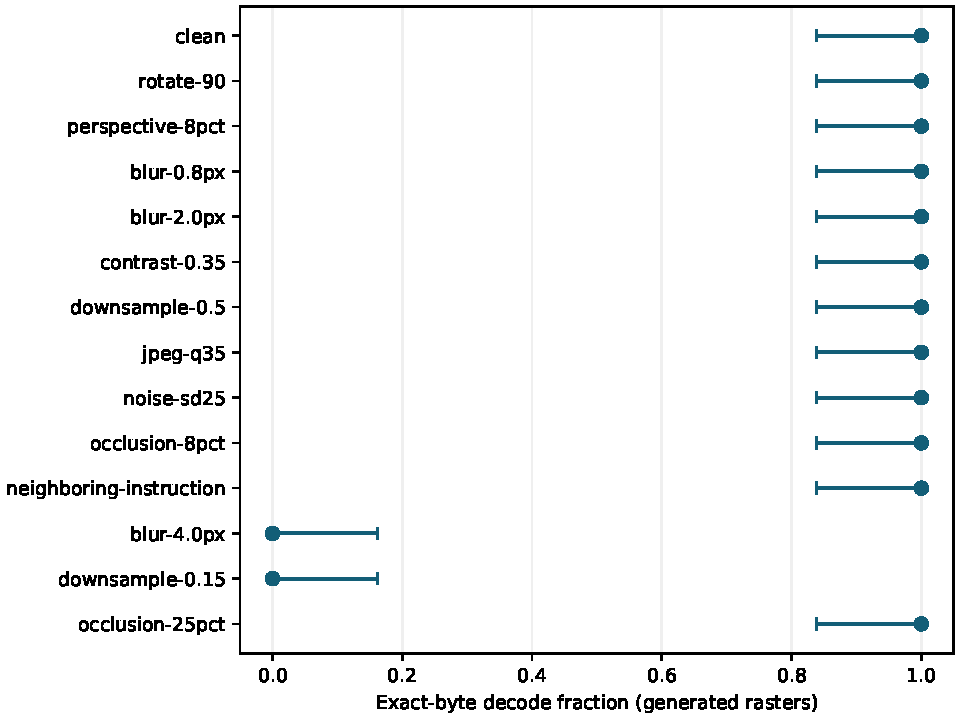
\includegraphics[width=0.85\textwidth]{artifacts/channel.pdf}
\caption{Exact-byte recovery on generated rasters, 20 source images per condition.
Bars are descriptive 95\% Wilson intervals. Conditions share source markers; the
figure is not a camera study or a deployment-security estimate.}
\label{fig:channel}
\end{figure*}

Clean images decoded in \CleanSuccesses{}/\BenchTrials{} trials, with median
\CleanMedian{} ms and p95 \CleanPninetyfive{} ms. Severe 4-pixel blur and 15\%
resizing failed in the recorded suite. The remaining conditions recovered all
recorded markers, without a successful decode yielding different bytes. These
results describe this codec, marker density and generated image family; they do
not generalize to arbitrary cameras, lighting, perspective or materials. A 20/20
condition still has a wide Wilson interval and is not a universal reliability
claim. The neighboring-instruction case demonstrates byte isolation only; no
language model interprets the instruction panel.
\subsection{Policy controls and schedules}
The serial suite repeats every named case \BenchTrials{} times with fresh keys,
challenges and temporary SQLite state. It includes changed principals, actions,
resources, purposes and arguments; altered signatures; unconfigured keys; session
and nonce transplantation; wrong audience; expired challenges and grants; grant
and issuer revocation; unregistered permission; wrong grant scope/modality;
consumed replay; malformed observation profiles; unsupported guarantees and
unaccepted assumptions. Modality-specific cases extend this common taxonomy.

An intentionally weak signature-only ablation ignores scope, freshness and
permission. It isolates why authentication alone is insufficient; its failures
are not evidence against correctly configured existing authorization. An equally
expressive sequential typed-policy control separately checks the same expected
challenge, action, supported guarantees and permission state. It shares
cryptographic and modality validators with the gateway and is not an independent
audit, full IFC implementation or reimplementation of published agent defenses.

The concurrency suite runs \BenchTrials{} trials of eight duplicate attempts
released together; each must produce exactly one receipt. Another
\BenchTrials{} trials hold the write boundary, revoke the grant and then release a
worker's commit. Every such prior-revocation schedule must produce zero receipts.
This is a deliberately selected serialized order, not an exhaustive scheduler
exploration. Tests also check rollback, expiry at the boundary and replay after
restart.

\subsection{Interpretation}
Across \SecurityObservations{} serial case observations
(\SecurityCases{} cases per trial), the gateway produced
\UnauthorizedEffects{} unauthorized new local receipts and
\TypedDisagreements{} disagreements with the typed control. The weak
signature-only check accepted \SignatureFalseAccepts{} observations that violated
the specified policy. Mixed accepted/denied gate processing had median
\GateMedian{} ms and nearest-rank p95 \GatePninetyfive{} ms. These one-host
measurements include SQLite work for accepted requests, but are not a matched
latency comparison with the control or an end-to-end physical delay.

Two limitation cases deliberately accept valid structured responses: transparent
live forwarding when no proximity guarantee is required, and a configured
attester producing a plausible report when sensor truth is not required. These
are modeled traces, not physical relay or compromised-device experiments. Requiring
proximity or consent is separately denied. Denial is not a result demonstrating
those properties. Channel trials and policy cases are distinct suites; the
runnable demos combine channel parsing, signature appraisal and effect insertion.

\subsection{Validity and missing comparisons}
Fresh source markers provide trial variation, but condition order is fixed and
all timing runs share one host. No matched comparison with a static signed-code
codec, authenticated API or physical-factor system is reported. The dataset is
small, synthetic and selected by the implementation authors. We release all
case rows and failures rather than interpreting zero observed policy violations
as a deployment attack probability. A future study needs camera/display trials,
physical relays, held-out scenes, independent review and agent-level disclosure
metrics across every enabled output.


\section{Discussion and Next Steps}
\paragraph{Fresh response is not physical association.}
The random challenge prevents replaying an unchanged old signed envelope into a
new stored interaction. It cannot prevent forwarding that challenge to a genuine
remote display and returning the response. Likewise a configured display may
assert the wrong resource or false status. Contracts requiring proximity,
resource-to-scene association or human consent are therefore unsupported and
must remain so after any modality handoff.

\paragraph{What is reusable.}
Exact-action snapshots, separate grant signers, bounded parsers and one-use local
receipts form a small engineering reference. They can be useful without being
new security primitives. A sequential policy with the same evidence and
requirements matches the measured decisions. Future work must compare equally
expressive controls when evaluating acquisition scheduling, integration effort
or useful autonomy; weakening the baseline is not an acceptable novelty argument.

\paragraph{Toward composition.}
OpenAVT independently protects structured messages carried through audio;
OpenATT appraises controller contact reports. Sharing a key, principal or project
name does not make their guarantees interchangeable. A future composition layer
must retain the exact claim, purpose, episode and dependencies and invalidate
support when those change. The current gateway accepts one modality per receipt
and does not implement that composition calculus, voice integration, evidence
reuse scheduler or AgentCore/Cedar deployment.

The next practical steps are an authenticated display enrollment flow, isolated
capture workers, camera/display trials and a participating backend with explicit
remote-effect semantics. Those steps are required to assess deployment rather
than merely extend a synthetic benchmark.


\bibliographystyle{plainurl}
\bibliography{references}
\appendix
\section{Open Science and Reproduction}
Artifacts include source packages, SDK examples, CLI demos, tests, raw benchmark
JSON, per-case timings, dependency versions and measured source hashes. Report
generators derive manuscript numbers from the JSON; the evidence checker verifies
arithmetic and source hashes. Public synthetic fixtures are separate from trials.

Using Python 3.11 or later, install the local core and modality package, then run
the demo, tests, 20-trial benchmark, report generator and paper Makefile. READMEs
provide exact commands and dependencies. Fresh keys change byte hashes and timing;
scenario seeds and transformations are explicit. No PyPI publication is asserted.

\section{Ethics and Deployment Limits}
Fixtures are generated, without people, customer records or private keys. The
sole effect is a local receipt. No hardware, LLM, cloud deployment or independent
security review was evaluated. Deployment needs authenticated enrollment,
protected keys and justified capture/effect semantics. This research draft is not
a submitted paper, new cryptographic primitive or formal security proof.

\end{document}
